%% content.tex
%%
\chapter{Content}
\label{ch:content}

To show the ``Heisenberg Effect'' a study design based on the work done by Pavlovych and Stuerzlinger~\cite{pavlovych_tradeoff_2009} was set up. The foundation of the study was a simple distal pointing task. This section gives an insight into the underlying implementation and considerations for the used study design. The experiment and the procedure are also described in detail. 

\section{Implementation}
\label{sec:implementation}

\subsection{Setup}
\label{subsec:impl:setup}

For the study, it was used the HTC Vive PRO and Unity with Steam VR to create the study setup. The controller for the HTC Vive PRO has a trigger at the bottom to click and select targets. To stay near the real devices, this trigger was used as the main button. The implementation is described in detail in the next sections. Based on the environment with Unity, C\# was used as the main programming language.
In the room in which the study was performed, it was built up two tracking sensors, to capture most of the room. In the center of the room stood a chair, fixed on the ground. An HTC Vive Pro headset and one controller were used in the demonstration. The user stood on the predefined spot in front of the chair or sit on it. 

\subsection{First attempts}
\label{subsec:impl:first_attempts}

The goal of the study was to find possible effects and evidence for the ``Heisenberg Effect''. As the effect described in a previous section (Subsection~\ref{subsec:related-work:defining-heisenberg-effect:description}), it was necessary to create a point and aim application for measuring the overall movements and hits, performed by the study subjects. Even at the beginning of implementation, it was clear to collect data of clicks out of the movement and in a static position. The aim of these two scenarios was to find and show differences in clicks out of motion and resting clicks (the clicks out of motion were discarded because of too many disturbances). Resulting from this specification, it was created a procedure for a single target task:

\newpage

\begin{enumerate}
    \item Show one target
    \item Wait for first click (not necessarily on target) - arising out of the movement
    \item Show counter if the user is on target and wait for the counter to finish
    \item Wait for second click (also not necessarily on target)
    \item Hide the target and begin again with the next one
\end{enumerate}

With this specification, it was possible to observe differences in static and motion-based clicks. This specification was transferred into the final implementation.
\newline
\newline
After solving the problem of the procedure, it was necessary to clarify how to arrange the targets on the canvas. The first attempt in implementation was to show a grid-based target layout (as shown in Figure~\ref{fig:layout-attempts} (a)).

\begin{figure}[h]
    \centering
    \subfigure[First layout attempt with grid based layout]{{\includegraphics[width=.4\linewidth]{graphics/grid.pdf}}}
    \qquad
    \subfigure[Grid based attempt in first implementation. After finishing the trial (with only three targets) the result is shown (the green points show the position of the raycast when the user clicked.)]{{\includegraphics[width=.5\linewidth]{graphics/in_app_graphics/heisenberg_before_end_small.pdf}}}
    \caption{Different Layout attempts}
    \label{fig:layout-attempts}
\end{figure}

The targets were displayed, one after another, on a three-by-four grid (three in height and four in width). Depending on the grid layout, there were three possible ways to display the targets one after another: 

\begin{enumerate}
    \item Show them in a static order
    \item Show them in a random order
    \item Create different static orders and rotate through them randomly
\end{enumerate}

The first layouts and experiments were based on this grid. After some testing (one of the results of the test runs is shown in Figure~\ref{fig:layout-attempts} (b)), there were some issues with this type of grid layout: The distances between the targets were different, caused by the three-by-four grid. Also, no other studies used such a grid layout for testing accuracy in pointing tasks. After some research, the paper by Pavlovych and Stuerzlinger~\cite{pavlovych_tradeoff_2009} showed some usable target layout. They used a Fitts' Law based circle task to test accuracy in their pointing tasks, which was adopted to this setup (see ~\ref{subsec:impl:circle_task}).
\newline

Based on the used setup (\ref{subsec:impl:setup}), the software should also handle most of the functionality the controller and the system supported. The controller supported six degrees of freedom (free position in three dimensions, plus three-dimensional angles). To portray also results for controllers with three degrees of freedom (fixed position, but three-dimensional angles), a mode for switching between these variations was implemented. 

The controller uses a  trigger to measure clicks. These clicks are not binary, meaning the strength of a press on the trigger can be measured by decimal values between 0.0 (trigger not touched) and 1.0 (trigger fully pressed). In the implementation, these values get also tracked to see, when a user initialized the click by slightly pressing the trigger, and when the click is really registered as a click by the implementation.

Besides the mode for degrees of freedom, the implementation handles two different modes, to create more variety in the study setup. The position of the user's arm (stretched out or applied to the body) and the position of the user itself (standing or sitting) is also tracked.

\begin{figure}[h]
    \centering
    \subfigure[Circle layout (the user was shown only one target at a time)]{{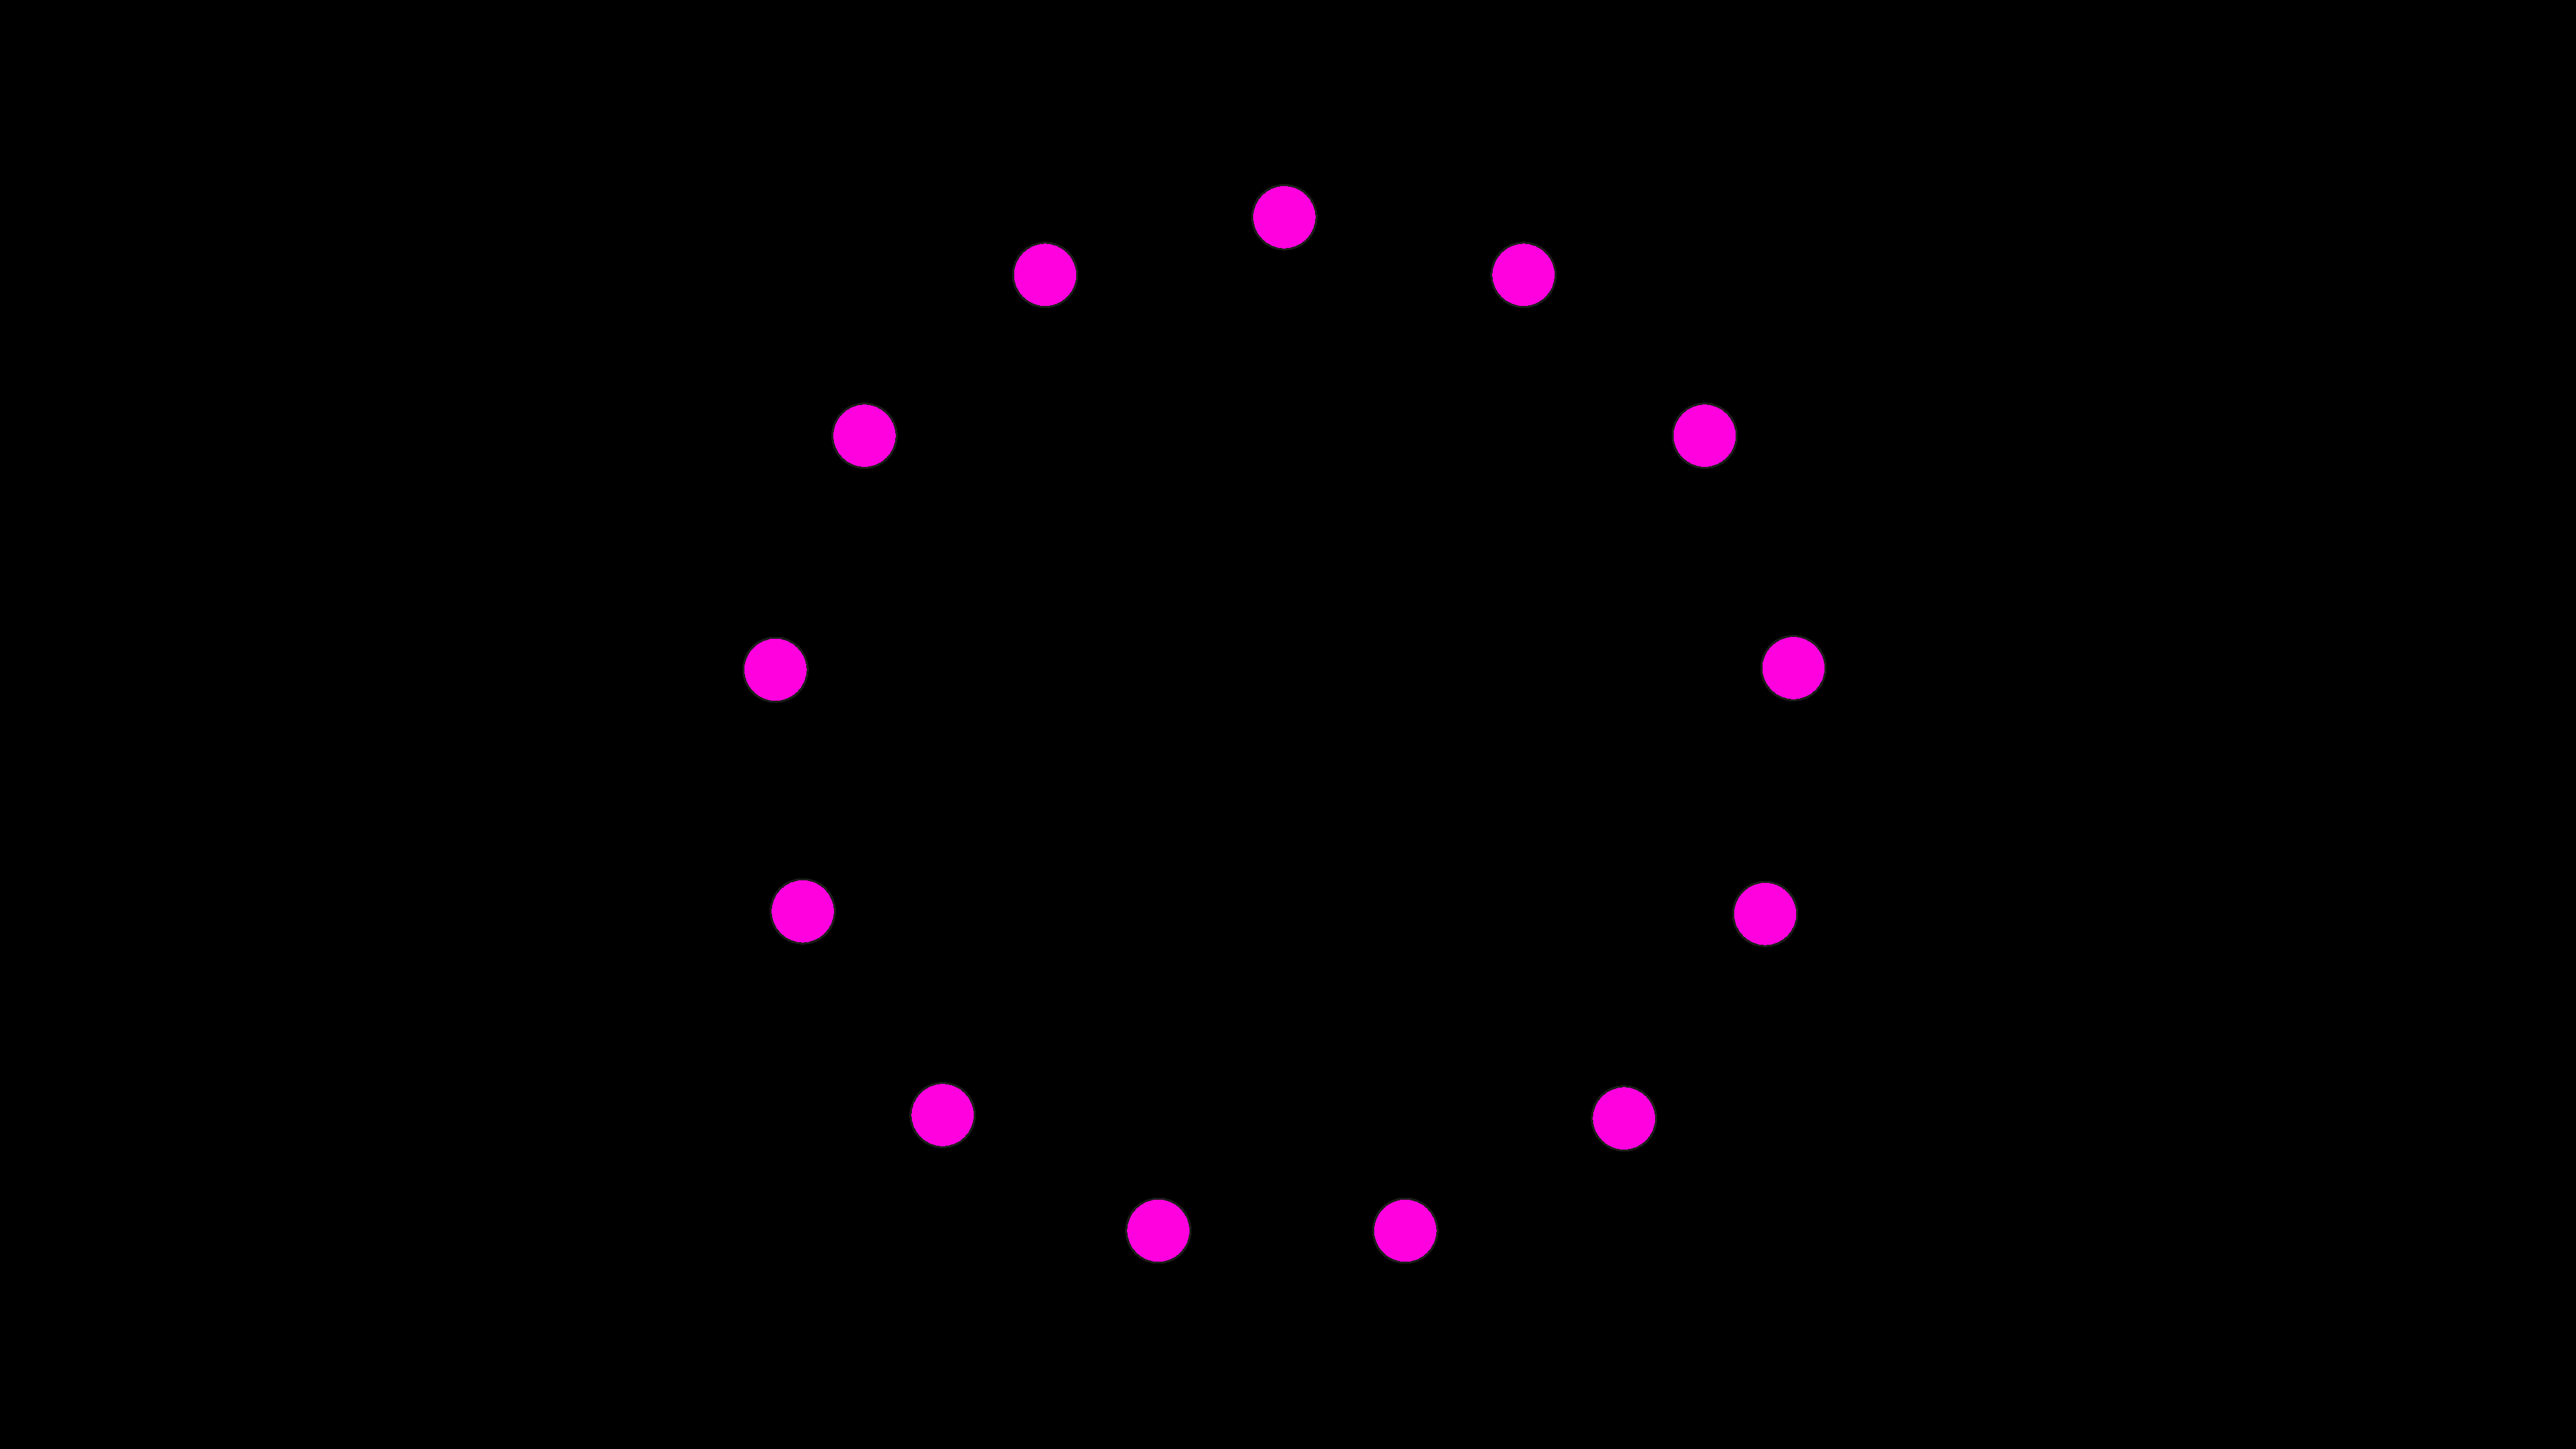
\includegraphics[width=.4\linewidth]{graphics/fitts_law_circle_in_app.pdf}}}
    \qquad
    \subfigure[Single target in real application]{{\includegraphics[width=.5\linewidth]{graphics/in_app_graphics/heisenberg_final_click_small.pdf}}}
    \caption{Final implementation}
    \label{fig:layout-final-implementation}
\end{figure}

\begin{table}
    \centering
    \begin{tabular}{c | c | c}
    \toprule
    Width & Amplitude & ID \\
    \midrule
    15  & 150   & 3.46 \\
    15  & 350   & 4.60 \\
    30 & 150 & 2.58 \\
    30 & 350 & 3.66 \\
    50 & 150 & 2.00 \\
    50 & 350 & 3.00
    \end{tabular}
    \caption{Used Index of Difficulty}
    \label{tab:id_values}
\end{table}

\subsection{Fitts' Law based circle pointing task}
\label{subsec:impl:circle_task}

Based on the experience made with a grid-base pointing task (described in section above: ~\ref{subsec:impl:first_attempts}), it was clear to use a Fitts' Law based circle pointing task as described by Soukoreff and MacKenzie~\cite{soukoreff_towards_2004}. To get a wide range of difficulties in the study, the \textit{ID} was calculated with different numbers of \textit{Amplitude} and \textit{Width} to get diverse \textit{ID}'s as described in Table~\ref{tab:id_values}.

On the basis of the \textit{Width} and \textit{Amplitude} values, described in Table~\ref{tab:id_values} for each \textit{ID} value was created an own Fitts' Law based circle pointing task.  In consideration of the study setup by Pavlovych and Stuerzlinger~\cite{pavlovych_tradeoff_2009} each circle war created with 13 targets (in consideration, that the first target cannot be evaluated, thanks to the unknown starting point). To calculate each point on the circle as a vector, the software iterates through the points from 0 to 12 (as \textit{i}) and uses the following formula:

\begin{align}
    \begin{bmatrix}
        x \\
        y \\
        z \\
    \end{bmatrix} &= \begin{bmatrix}
                        (Amp / 2) \cdot \sin(i \cdot (360 / 13)) \cdot (\pi / 180) \\
                        (Amp / 2) \cdot \cos(i \cdot (360 / 13)) \cdot (\pi / 180) \\
                        0
                     \end{bmatrix}
\end{align}

The size (\textit{Amp}) of the target was implemented later when each point was shown on the canvas. A sketch of the circle is shown in Figure~\ref{fig:pointing_task}. The Figure~\ref{fig:layout-final-implementation} shows the circle layout in implementation (a) and a single target with a raycast in the application.

\begin{figure}[h]
    \centering
    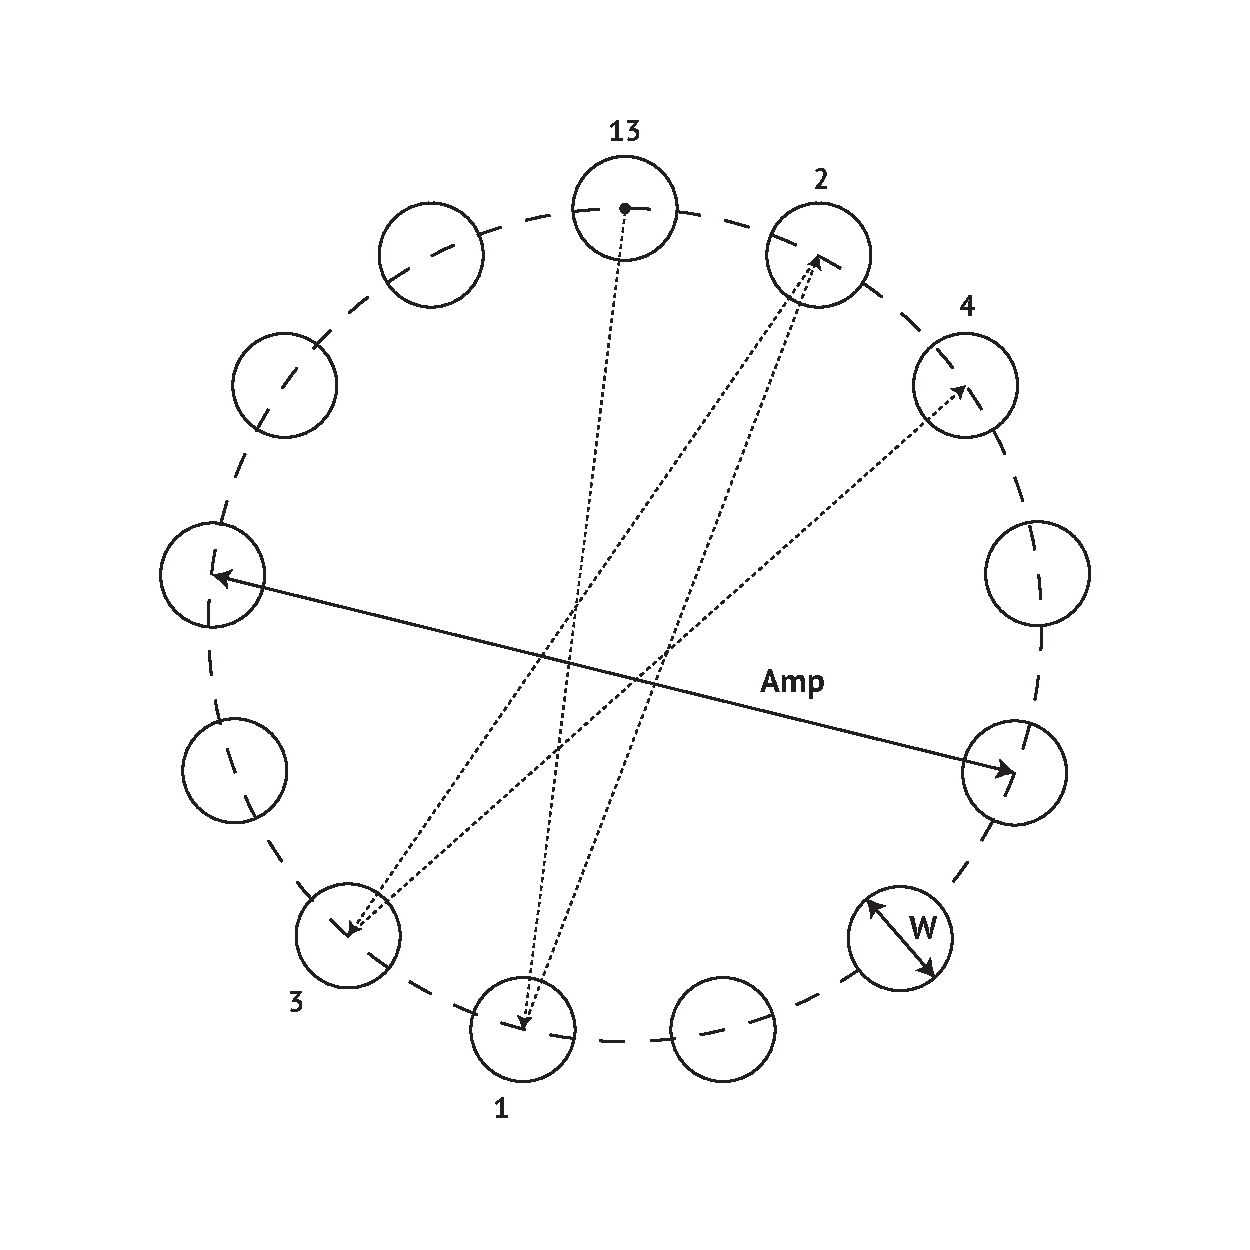
\includegraphics[width=.7\columnwidth]{graphics/fitts_law_circle.pdf}
    \caption{Multidirectional pointing \& clicking task}
    \label{fig:pointing_task}
\end{figure}

\subsection{Study implementation}

On the basis of the previous discussions, the software was implemented to run the study with participants. There are 8 rounds (2 body positions, 2 arm positions, 2 degrees of freedom = 8 possibilities) for each participant, which differ in the following modes:

\begin{table}[h]
    \centering
    \begin{tabular}{|p{5cm}||p{3cm}|p{3cm}|}
    \hline
    arm position & stretched out & applied to the body \\
    participants position & standing & sitting \\
    controller degree of freedom & 3 & 6 \\
    \hline
    \end{tabular}
    \caption{Task modes}
    \label{tab:task_modes}
\end{table}

Each of these rounds contained six Fitts' Law circles, based on the six different \textit{ID} values for width and amplitude calculated in Table~\ref{tab:id_values}. The modes mentioned in~\ref{tab:task_modes} and the previously mentioned circles were combined with the help of Latin Squares. These Latin Squares were used to give each participant a different sequence of modes and of circles. The implementation calculated the two of these Latin Squares. One to iterate through the different possible combinations of arm position, body position and degrees of freedom. The other one was used to iterate through the possible amplitudes and sizes of the Fitts' Law circle task. Both are based on a unique user id, so the iterations are steady.

\subsection{Design}
\label{subsec:design}

Resulting from the previous research and testing, the experiment had five different and independent variables in a 2 x 3 x 2 x 2 x 2 arrangement (makes a total of 48 combinations):

\begin{itemize}
    \item Target amplitude: 350 and 150;
    \item Target width: 15, 30 and 50;
    \item Arm position: stretched out and applied to body;
    \item User position: standing and sitting;
    \item Degrees of freedom: 6 and 3;
\end{itemize}

Based on these numbers, each participant had to complete 48 Fitts' Law circles with each 13 recorded targets and two clicks each target. Given the 16 subject participating of this study, it results in a total number of $16 \cdot 48 \cdot 13 \cdot 2 = 19,968$ trials.

\subsection{Tracking device jitter}
\label{subsec:basic_jitter}

To eliminated device jitter, the position of the controller and headset were tracked in a total static position (headset on a table and controller on the floor). The controller and headset showed fluctuations in position, even when in a total static position. The results were used in Subsection~\ref{subsec:evaluation:clearing_the_data:device_caused_jitter} to clear the data from the device-caused jitter.

\subsection{Source Code}
\label{subsec:source_code}

The full source code and all assets can be found in a GitHub repository\footnote{\url{https://github.com/mc17uulm/Heisenberg}}. Under $assets/HeisenbergScene/Scripts$ all relevant scripts can be found. The script $Processing.cs$ is the entry point for the application.

\section{Experiment}
\label{sec:experiment}

\subsection{Participants}
\label{subsec:participants}

All of the sixteen participating subjects were actual or former students of the Ulm University. The ages of the participants reached from 20 to 30 years (by an average age of 24.5 years). The group of participants consisted of into 8 male, 7 female, and one other. 15 out of 16 subjects were right-handed. 7 out of 16 had visual aids.

Most of them had already experience with virtual reality: 13 of 16 participants used VR at least once, 11 out of 16 had even more than one month of experience in VR. Half of the subjects used VR frequently. The subject also got asked if they ever used games in VR, where pointing and shooting is the main task. Half of the subjects reported so. When to judge their skills, the subjects reported an average value of 2.5 (by a scale from 1 to 5; 1 is basic and 5 is skilled). 

The duration of the study was 40 minutes to one hour, mostly based on the pointing skills and strategies of the participants. 

\begin{figure}[h]
    \centering
    \subfigure[User is standing with stretched out  arm]{{\includegraphics[width=.4\linewidth]{graphics/standing.pdf}}}
    \qquad
    \subfigure[User is sitting with stretched out arm]{{\includegraphics[width=.4\linewidth]{graphics/sitting.pdf}}}
    \caption{Body positions in study}
    \label{fig:body_positions}
\end{figure}

\subsection{Procedure}
\label{subsec:procedure}

The user held the controller in his dominant hand and was able to interact via a click on the trigger. After the user read the task (Task description illustrated by Figure~\ref{fig:procedure-design} (c)) and changed his arm and/or body position he could start the round by clicking the trigger. By starting a round, all controller positions, rotations, and clicks were tracked and logged. Between these rounds, the user had the change to have a small break and rest his arm.

Each of these eight rounds showed one target at a time. The user had to direct his controller to the target (the user could see where he was pointing by a raycast) and click for the first time. This click was called the ``ballistic click'' because it resulted out of the motion. It wasn't necessary for the click to be on target. The data should show where the user aimed to and where he finally ended when clicking the trigger. For the second click, the user had to be on target for at least 500 milliseconds (illustrated by a timer turning from red to green - example in Figure~\ref{fig:procedure-design} a \& b). This second click was called ``static click``. The click in this position was necessary to compare the differences between a click out of motion and one out of a static pointing on the target. 

All targets were placed on a circle, which implemented a standard Fitts' task. But only the actual target was shown to the user. After the two clicks on one target, the next target was shown.

\begin{figure}[h]
    \centering
    \subfigure[Timer is running]{{\includegraphics[width=.25\linewidth]{graphics/in_app_graphics/heisenberg_final_click_filling_small.pdf}}}
    \qquad
    \subfigure[Timer is finished and user has to click]{{\includegraphics[width=.25\linewidth]{graphics/in_app_graphics/heisenberg_final_click_filled_small.pdf}}}
    \qquad
    \subfigure[New task is shown to the user. In between these tasks the user could rest]{{\includegraphics[width=.25\linewidth]{graphics/in_app_graphics/heisenberg_final_task_small.pdf}}}
    \caption{Procedure in real application}
    \label{fig:procedure-design}
\end{figure}

\section{Collected Data}
\label{sec:results}

The software saved all tracked data in csv files (\textbf{c}haracter \textbf{s}eperated \textbf{v}alues) for each user. Following values get tracked:

\begin{itemize}
    \item Identification of the user (only an id to match with the demographic data)
    \item Standard information about the task (arm and body position; degrees of freedom; a timestamp)
    \item Events and system states (pressed trigger, click, etc.)
    \item Strength of pressure on the trigger (value between 0 and 1)
    \item Position and size of the target
    \item Position and rotation of the controller
    \item Position of pointer on canvas
\end{itemize}

These values were tracked and saved for each frame. To ease the evaluation of the data (all of the tracked data for one participant ranged from 20 megabytes (MB) to 45 MB.), the software produced two extra log files. In one of them, the point of first press and click were selected and the difference between them calculated and saved. In the other one, the software saved the calculated \textit{Throughput} and the values (\textit{Effective Width}, \textit{Effective Distance}, \textit{Effective ID}, \textit{Effective Throughput} and \textit{Mean Movement Time}) based on the model of the Extended Fitt's Law, explained in Section~\ref{subsec:related-work:background:extended_fitts_law}. So each trial with on participant ended with three anonymous log files.

